\documentclass{beamer}
\usepackage{pgfpages}
\usepackage{newtxtext,newtxmath} %time new roman
%\setbeameroption{show notes}
%\setbeameroption{show notes on second screen=right}
\usetheme{Warsaw}
\usepackage[french]{babel}

\usepackage{tikz}
\pgfdeclareimage[height=0.5cm]{le-logo}{}
%\setbeamertemplate{footline}[frame number]
%Set number slide
\usepackage[backend=biber, natbib, maxbibnames=20, citestyle=authoryear]{biblatex}
\addbibresource{handwritten.bib} 
\usepackage{multirow}% row fusion
\usepackage{array} % column fusion
\usepackage{xfrac} % small fractions
\usepackage{adjustbox}
\usepackage{listings}
\usepackage{color}
\definecolor{gray}{rgb}{0.4,0.4,0.4}
\definecolor{darkblue}{rgb}{0.0,0.0,0.6}
\definecolor{cyan}{rgb}{0.0,0.6,0.6}
 \titlegraphic{\vspace{-1cm}
      
\includegraphics[width=2.5cm]{images/paris8_1}\hspace*{4.75cm}~%
      \hfill
      
\includegraphics[width=2.5cm]{images/logo}
}
\setbeamertemplate{frametitle}{\nointerlineskip  
    \begin{beamercolorbox}[wd=\paperwidth,ht=2.75ex,dp=1.375ex]{frametitle}
        \hspace*{2ex}\insertframetitle \hfill {\small\insertframenumber/\inserttotalframenumber} \hspace*{1ex}%
    \end{beamercolorbox}}

\usecolortheme{wolverine}
\setbeameroption{hide notes} % Only slides


%%%%%%%%%%%%%%%%%%%%%%%%%%%
\title[KNN] 
{K-Nearest Neighbor}
%\subtitle {ne compléter que si l'article possède un sous-titre}
\author[Komlan Dantodji] 
{Komlan Jean-Marie DANTODJI}

\institute[]
{
  Etudiant en M1 Big Data
  \and
  Université Paris 8}
\date{27 novembre 2020}


\begin{document}
\begin{frame}
  \titlepage
\end{frame}

\begin{frame}{Plan}
  \tableofcontents
\end{frame}
\section{Introduction}
%\subsection{Linéarité séparable}
\begin{frame}{Structure globale des algorithmes du machine learning }
	\begin{figure}[H]
    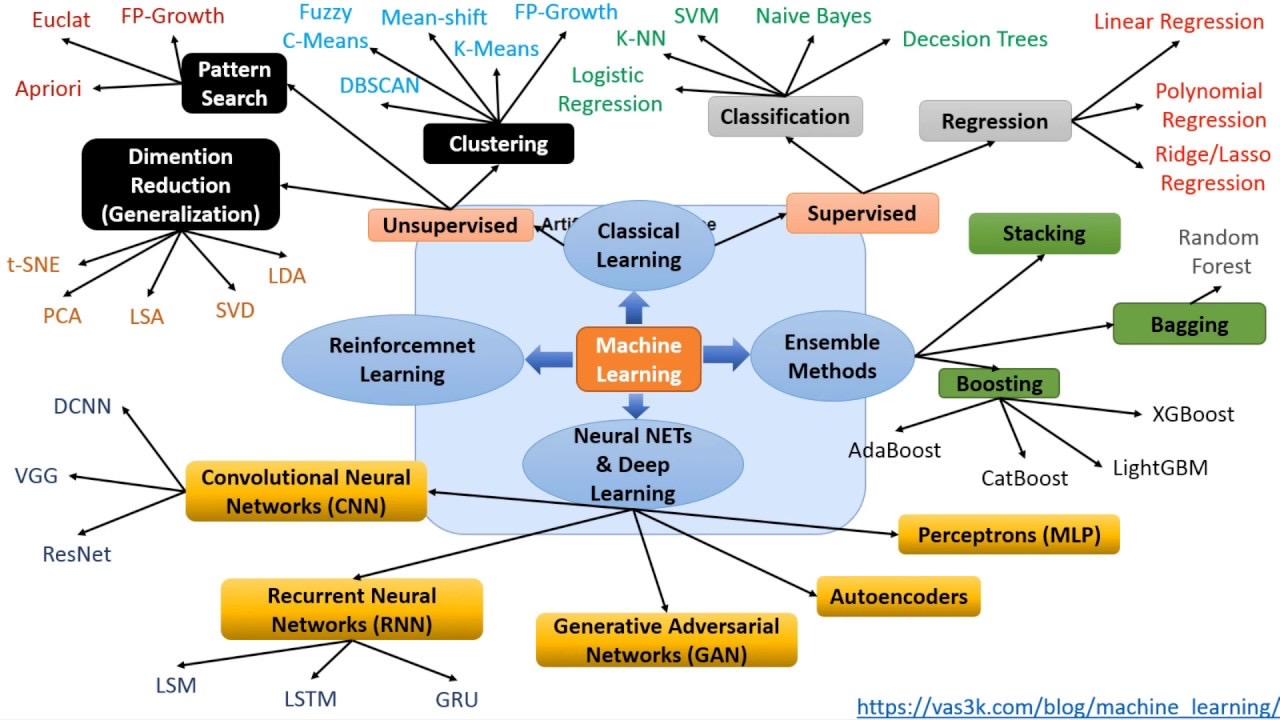
\includegraphics[width=\linewidth,height=5.8cm]{images/AI_fieds.jpg}
    \caption{Structure du machine learning}
    \label{fig:L1}
\end{figure}
\end{frame}

\section{K-Nearest Neighbor}
\subsection{Préparation des données}
\begin{frame}{Préparation des données}
\begin{itemize}
		\item Base de donnée
		\item Traitement préalables nécessaires
\end{itemize}
\end{frame}
\subsection{Fonctionnement du K-NN}
\begin{frame}{Fonctionnement du K-NN}
\begin{figure}[H]
    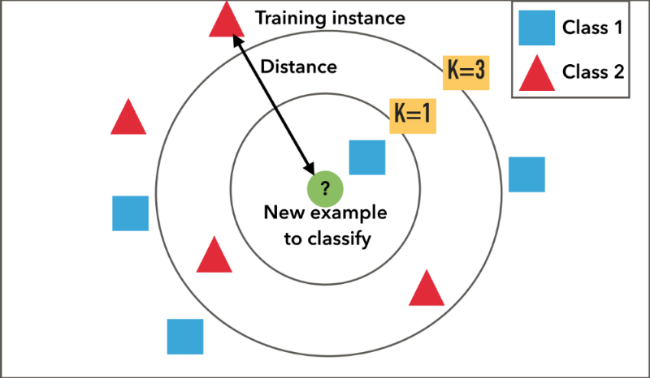
\includegraphics[width=\linewidth, height=5cm]{images/knn_sheama.png}
    \caption{K-Nearest Neighbor}
    \label{fig:L1}
\end{figure}
\end{frame}
\subsection{Distances}
\begin{frame}{Les types de distances}
\begin{itemize}
		\item Distance euclidienne
		$$d(A,X) = \sqrt{\sum_{i=1}^{n} (a_{i}-x_{i})^{2}}$$
		\item Distance de Manhattan\\
		$$d(A,X) = \sum_{i=1}^{n} \mid{a_{i}-x_{i}}\mid$$
		\item Distance de Minkowski
		$$d(A,X) = \sqrt[p]{\sum_{i=1}^{n} \mid{a_{i}-x_{i}}\mid^{p}}$$
\end{itemize}
\end{frame}
\subsection{Choix du paramètre K}
\begin{frame}{Choix du paramètre K}
\begin{itemize}
		\item Utilisation de K
		$$K=\sqrt{nombre-de-donnees }$$
		\item Choisir K suivant celui qui donne une meilleure prédiction
\end{itemize}
\end{frame}

\subsection{Algorithme en Python}
\begin{frame}{KNN implémenté en Python}
\begin{figure}[H]
    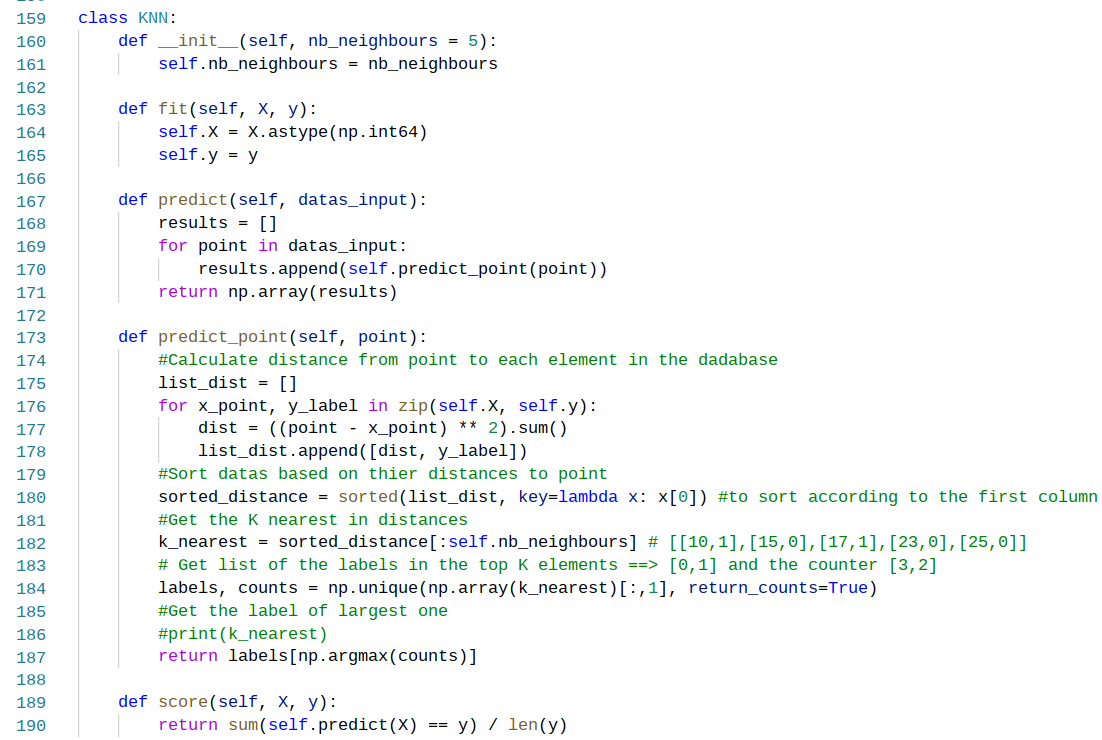
\includegraphics[width=\linewidth, height=5.8cm]{images/knn_in_python.png}
    \caption{KNN en python}
    \label{fig:L1}
\end{figure}
\end{frame}

\section{Applications}
\subsection{Domaines d'application}
\begin{frame}{Domaines d'application}
\begin{itemize}
		\item Ecriture manuscrite
		\item En médécine, prédire des maladies
		\item Classification des images
\end{itemize}
\end{frame}

\section{Conclusion}
\subsection{Conclusion}
\begin{frame}{Avantages et désavantage du K-NN}
\begin{enumerate}
		\item Avantages du KNN\\
		\begin{itemize}
		\item Facile à comprendre
		\item Apprentissage rapide
		\end{itemize}
		\item Désavantage du KNN\\
		\begin{itemize}
		\item Limité à partir d'une large donnée d'apprentissage
		\item La valeur de K optimal non connu au préalable
		\end{itemize}
	\end{enumerate}
\end{frame}
\section{Références}
\begin{frame}{Références}
[1] Audibert, J.Y. , Tsybakov, A.B. (2007) Fast learning rates for plug-in classifiers under the margin condition", Ann. Statist, 35: 608 633.\newline
[2] Bailey, T. Jain, A. (1978) A note on distance-weighted k-Nearest Neighbor rules, IEEE Tra, Systems, Man, Cybernetics, 8: 311-313
\end{frame}
\section{}
\begin{frame}{}
 \begin{block}{}
  \centering
  Merci pour votre attention
  \end{block}
\end{frame}

\end{document}